%%%%%%%%%%%%%%%%%%%%%%%%%%%%%%%%%%%%%%%%%%%%%%%%%%%%%%%%%%%%%%%%%%%%%%%%%%%%%%%%%%
%%% Introduction
%%%%%%%%%%%%%%%%%%%%%%%%%%%%%%%%%%%%%%%%%%%%%%%%%%%%%%%%%%%%%%%%%%%%%%%%%%%%%%%%%%
\chapter{Introduction}
	\label{ch::introduction}
	
	\begin{figure}[h!]
		\centering
		\fbox{\includegraphics[width=\textwidth]{on_the_rocks2.jpg}}
		\caption{The BlueFoot Quadruped Robot}
		\label{fig::bluefoot_glamour}
	\end{figure}
		The design of legged robots and associated methods of locomotion control has been an area of interest spanning the past several decades, as shown by \cite{McGhee1965,Hodgins1991,Altendorfer2001,Kolter2008,Wieber2015}. Quadruped robotic systems have gained popularity in studies pertaining to variable terrain navigation and full-body stability adaptation. Well known examples of this from the past 15 years are the Tekken \cite{Fukuoka2003}, Kolt \cite{Estremera2006}, BigDog \cite{BigDog2008}, and HyQ \cite{Semini2010_PHD} quadrupeds. Many of these systems have been implemented on a larger scale so that they can carry substantial payloads while maintaining adequate system bandwidth for fast gaits and robustness to rough terrains. Few, however, have been implemented on the scale of a hobby-robot platform while still maintaining an aptitude for rough terrain navigation and comparable sensory prowess.

		The BlueFoot quadruped is a self-contained, fully-actuated platform with the dexterity to perform stabilization and repositioning maneuvers on variable terrains along the same lines as the LittleDog platform \cite{Rebula2007}. Namely, BlueFoot has been designed with 16 actuated degrees of freedom to allow for the execution of a wide range of body and leg articulations. Moreover, BlueFoot's range of articulation allows it to take on a large range of poses during motion. This level of dexterity grants the BlueFoot platform the several notable abilities. For one, it can overcome raised terrain, allowing it to traverse uneven terrain. Additionally, BlueFoot can articulate (\IE pitch and yaw) its on-board vision sensors array, which is attached to its main trunk, by reposing its body through using aggregate leg motion controls. BlueFoot also includes a sizable array of other on-board sensors for feedback and control, including joint position, velocity and loading sensors; an inertial measurement unit (IMU); and foot-contact sensors. Using the computational, sensory and motor capacities at hand, BlueFoot has the ability to utilize similar control mechanisms to those implemented on larger quadruped systems. 

		The BlueFoot platform inherently demands a variety of control routines to achieve locomotion and system stability, making this robot an ample platform for studies related to gait design and motion planning. In particular, BlueFoot's controller considers the systems kinematic model; and involves open-loop gait design and stabilization for the purpose of achieving dynamic locomotion control. In particular, BlueFoot is gaited via a central pattern generator (CPG) based gaiting technique which is augmented with a foothold controller along the same lines as \cite{Ajallooeian2013} and \cite{Rutishauser2008}. Additionally, active platform stabilization is performed via a zero-moment point (ZMP) based body placement controller which stabilizes the system during arbitrary gaiting sequences. The controllers presented here make use of virtual-forces to drive system reference commands and make significant use of the system's forward kinematic model for the purpose estimating the positions of the robot's joints and feet. Finally, outer-loop control routines are implemented to supply commands and corrections used in system navigation control. Among these controllers are a potential fields navigation controller which incorporates image features as target-points to track; and 3D point-cloud processing routines for surface reconstruction and foot-hold planning.

		\section{Central Pattern Generators for Gait Control}

		As previously mentioned, BlueFoot's core gaiting routine relies on the utilization of artificial CPG's, which are inspired from biological neural networks which generate rhythmic motions \cite{Ijspeert2008}. \cite{Arena2000} describes CPGs as a form of self-organizing cellular neural network, and also explains the a the role of limited feedback in CPG's. Infact, a key feature of these networks is that they can act without explicit feedback inputs, or even without directions from a higher-level command unit, such as a brain. Instead, signals emanating from independent motor units and feedback gathered from sensory neurons are utilized to trigger or inhibit a sequence of successive, self-coordinated motor operations. The activation sequences performed by a series of neural unit combine in phase-locked loops create cyclic motion patterns. In robotics, biological CPG's have inspired an artificial counterpart in which neural units are represented by multi-state unit-oscillator. The dynamics of these unit oscillators are coupled with other oscillators within the artificial CPG network. Typically, the CPG network is implemented on a controller, which numerically integrates the dynamics each neural oscillators. The output states of each unit-oscillator are used to drive selected degrees of freedom of a robot system through actuator reference-command signals. Oscillator outputs could also be used for planning periodic motions in the robot's task space, which are then translated into the joint-space via an inverse kinematics mapping, as is done in BlueFoot's gait control routine. The motions produced using the dynamical outputs of each unit-oscillator are usually coordinated through the careful tuning of oscillator coupling, which incurs particular phase offsets between the individual limit-cycles. This stable coordination between oscillators is what allows the CPG to be applied to the performance of a higher-level motor task, such as walking.

		Studies dealing specifically the application of CPG's to multi-legged robot gaiting (specifically quadruped, hexapods and octopodal robots) have been carried out by \cite{Arena2001,Klaassen2002,Arena2004,Inagaki2003,Inagaki2006,Billard2000,Brambilla2006,Buchli2006,Tsujita2001,Tsujita2004}.  In particular, \cite{Ijspeert2008} states that the attractiveness of CPG's in the control of legged robot locomotion lies in a resulting ability to decouple robot motor control, \IE walking, from higher-level planning. Additionally, CPG's offer an effective way for smoothly switching between gaiting patterns, \EG walking, trotting, or pacing, by simply modifying only a few control parameters. As a result, the use of CPG's greatly reduces the dimensionality of the gaiting control problem by generating coordinated motions which can be modified to yield different overall motion patterns without explicit modification of each degree of freedom employed in gait execution.

		An important aspect of the CPG-based gait design applied to the BlueFoot platform is the incorporation of feedback mechanisms which modify the aforementioned CPG parameters. The use of feedback to modify the CPG network for the purpose of improving gaiting stability was guided, in part, by the work of \cite{Fukuoka2003,Endo2004}. Namely, BlueFoot's CPG based gait generation incorporates inertial feedback signals into its CPG mechanism by using them to modify oscillator amplitudes and modulate unit-oscillator frequencies. Additionally, instead of using a CPG to control the outputs of individual quadruped joints, CPG outputs are mapped to stepping trajectories and foot-motion execution patterns. This approach yields a gaiting technique which combines the conveniences of CPG-based gaiting with the heightened control precision of explicit foot-step planning in the robot task-space. Moreover, foot-placement is explicitly prescribed via a separate planning mechanism which decoupled from the CPG gait controller. This method allows a CPG-based motion generation method to be applied gaiting over varying terrains.

		Because CPG-based gaits are inherently open-loop motion control routines, a combination of axillary mechanisms must be used in concert with the base CPG gait controller in order to ensure system stability during gaiting. The incorporation of feedback signals to modified CPG parameters aids in achieving this to some degree, but is usually insufficient for stable walking over largely uneven terrains. 
		
		Additionally this method would require very careful parametric tuning to work robustly under a larger variety of terrain conditions. Thus, other means of stabilization have been incorporated into BlueFoot's gaiting routine to aid in stability. In particular, BlueFoot's core stabilization routines make use of a concept formally named \emph{artificial synergy synthesis} in which gaiting is carried out independently of a stabilization control. Namely, body stabilization is performed by a restricted set of the robot's degrees of freedom while gaiting is carried out independently by the remaining \cite{Vuko1972,Yamaguchi1993}. In an original implementation of this technique, adaptations to trunk motion are utilized to stabilize the overall motion of the robot utilizing a ZMP-based approach, as is done here, while gaiting is controlled by a fixed-motion routine. Here, body and foot-placement are both controlled dynamically, but still independently. The outputs of each controller, which specify body and foot placement in the robot task space, respectively, are combined using the robot's inverse kinematics solution, which generates a final set of joint references.

		\section{Zero Moment Point Body Placement Control}

		The zero-moment point (ZMP), which is equivalent to the center of pressure (CoP), is formally defined as the point on the ground beneath a walking system at which the net moment acting upon the trunk (referred to as the tipping moment) is zero \cite{Sardain2004}. The concept of ZMP and its application to legged robotics was originally introduced by \cite{Vuko1972} and expanded upon in \cite{Goswami1999}, both of which describe ZMP theory towards use in the control of biped robots.

		Formally, the ZMP, $p_{ZMP}$, can be defined using a formulation for the CoP wherein the moments about $\tau_{x}$ and $\tau_{y}$, the tipping-moments applied to the robot's body in the world frame, are equal to zero. The solution for $p_{ZMP}\in\Re^{3}$, with respect to a set of $N$ foot contact points $p_{i,e}\in\Re^{3}$ and $N$ associated applied foot-contact forces $f_{i,e}\in\Re^{3}$, arises as a bounded set of solutions to the equation
			\begin{equation}
				\sum^{N}_{i=1}\wrap{p_{i,e}-p_{ZMP}}\times f_{i,e} 
				= 
				\left[
					\begin{array}{c}
						\tau_{x}	\\
						\tau_{y}	\\
						\tau_{z}
					\end{array}
				\right]
				=
				\left[
					\begin{array}{c}
						0			\\
						0			\\
						*
					\end{array}
				\right]
			\end{equation}
		where $z$-coordinate of $p_{ZMP}$, $\zcomp{p_{ZMP}}$, is strictly zero, as shown in \cite{Wieber2015}. This expression is derived from an inspection of the dynamics which govern the total angular momentum, $\dot{L}$, about the legged system's center of gravity (COG), $p_{COG}$:
			\begin{equation}
				\dot{L} = \sum_{i=1}^{N} p_{i,e}\times f_{i,e} - m_{T} p_{COG} \times \wrap{ \ddot{p}_{COG} + \vec{g} }
			\end{equation}
		where $m_{T}$ is the total mass of the legged system and $\vec{g}$ is the standard gravity vector. Assuming that all foot-contacts exist on a flat plane, \IE $\zcomp{p_{i,e}}=0\SSep \forall i=[1,...,N]$, and all contact force, $f_{i,e}$ are pointing upward, the $p_{ZMP}$ of the system can be written as
			\begin{equation}
				p_{ZMP} 
				= 
				\frac{ \sum_{i=1}^{N} \wrap{ p_{i,e} \times f_{i,e} } }{ \sbrack{\sum_{i=1}^{N} f_{i,e}}_{z} }
				= 
				\frac{ 	p_{COG} \times \wrap{ \ddot{p}_{COG} + \vec{g} } + \dot{L}m_{T}^{-1} }{ \zcomp{ \ddot{p}_{COG} + \vec{g} }}
				\in \emph{C}_{ZMP} 
			\end{equation}
		where
			\begin{equation}
				\emph{C}_{ZMP} = \convhull{p_{1,e},p_{2,e}...,p_{N,e}}
			\end{equation}
		with $\text{conv}(*)$ defining a convex hull from the  input points, $(*)$, and is used to represent the solution space of $p_{ZMP}$. Moreover, $\emph{C}_{ZMP}$ places a bound on the angular momentum $\dot{L}$ which results from contact variations presented through $p_{i,e}$ and $f_{i,e}$. Setting $\dot{L}=0$, we defined a condition for zero tipping. For BlueFoot's ZMP controller formulation, it is also assumed that the acceleration of the COG is sufficiently small, \IE $\ddot{p}_{COG}\approx0$ which yields the following, intuitive stability condition:
			\begin{equation}
				\norm{p_{ZMP} - p_{COG}} < \epsilon
			\end{equation}
		where $\epsilon\ll1$ is a small bounding constant. Thus, the general idea of this ZMP-based controller is to compute an approximate ZMP location and place the center of the robot's trunk (described by the translation $p_{b}$) such that the platform's COG approaches its associated ZMP for some arbitrary kinematic configuration, thus minimizing $\norm{\dot{L}}$ so as to avoid tipping.


		\section{Trunk stabilization}

		In addition to the aforementioned task-space controllers, a learning controller, which features the use of a NARX neural network is used to aid trunk stability has been studied. In essence, this controller learns to approximate disturbance dynamics during periodic gait routines and corrects trunk orientation by administering adaptations to joint position controls. The goal of such control routine is to achieve a level trunk during locomotion.
			
		A NARX-NN architecture is used in this controller because of  its known effectiveness in approximating nonlinear difference systems and making multivariate time-series predictions \cite{Tsungnan1996,ChenBillings1990,Hihi1996,Billings2013}. Moreover, the NARX-NNs is a natural fit for a problem of this nature where the dynamics being considered are both periodic and of a high enough complexity where a nonlinear approximation method is warranted. The parallel NARX-NN model, shown in Figure \ref{fig::narx_net}, is comprised of a feed-forward neural network whose input layer accepts a series of time-delayed system state values and network-output histories. The NARX-NN is trained to predict system states in the next time-instant from these inputs. Conveniently, NARX-NN training can be performed using standard BP because recurrence occurs between network inputs and outputs, and not within the hidden layers \cite{Nelles2001}.

		The NARX-NN is trained to capture the effects of forces and moments and dynamical couplings that act on the trunk so that an appropriate torque input to the joints is computed to reduce such effects on trunk orientation while performing the gate. This is achieved by considering the inverse dynamics corresponding to joint motion.

		Disturbances imparted upon the trunk during gaiting manifest in the term $\Phi$, largely as a result of variations in $f_{ext}$ and associated effects due to dynamical coupling. Because of this, the NARX-NN will learn an estimate for $\Phi$, denoted $\hat{\Phi}$. The network is trained on-line using the standard incremental back-propagation (BP) algorithm with an adapted learning rate, $\gamma^{lr}$ and momentum term, $\mu$ \cite{Rumelhart1988,Rumelhart1995}. This error BP algorithm is a gradient-descent based method used to train a feed-forward neural network with $n$-layers and layer-connection matrices $\setwrap{W^{1},W^{2},...,W^{n-1}} \in \emph{W}$. The BP algorithm, as used in this control approach, is summarized in matrix-vector form in (adapted from \cite{Rojas1996ch7}) as follows: 

		\begin{equation}
			\Delta W^{i} =
				-\gamma^{lr} \wrap{ \frac{ \partial o^{i} }{\partial {W^{i} } }  o^{i-1} }^{T}  + \mu \Delta W^{i} = 
				-\gamma^{lr} \delta^{i} \wrap{o^{i-1}}^{T}  + \mu \Delta W^{i}
			\label{eq::bp_weight_update}
		\end{equation} 
		%
		where
		%
		\begin{equation*}
			\delta^{i} = \wrap{ \nabla_{y} \sigma^{i}\wrap{y^{i}} } e^{i}
			\label{eq::bp_error}
		\end{equation*}
		\begin{equation*}
			y^{i} = W^{i} o^{i-1}
			\label{eq::bp_error}
		\end{equation*}
		\begin{equation*}
			e^{i} =  \wrap{ W^{i} }^{T} \delta^{i+1} \hspace{2mm} \forall \hspace{2mm} i\neq n,
		\end{equation*}
%%
		$\gamma^{lr} \in [0,1]$, the learning and  $\mu \in [0,1]$, the learning momentum; $W^{i} \in \Re^{N_{O}^{i}\times N_{I}^{i}}$, which represents the weighting matrix between the \Ith layer (of size $N_{I}^{i}$ nodes) and $(i+1)^{th}$ layer (of size $N_{O}^{i}=N_{I}^{i-1}$); $\Delta W^{i}$, which represents the corresponding weight update to $W^{i}$; and $e^{i}$ is the output error for each \Ith layer. For the output ($n^{th}$) layer, $e^{n}$ is equal to the difference between the network output and the network output target, which will be defined later. For all other layers, $e^{i}$ represents a \emph{back-propagated} error. from the $(i+1)^{th}$ layer.

%%
		$\sigma^{i}(y^{i})$ is a layer-wise activation function which outputs a vector of scalar activation outputs, $\sigma_{j}^{i}(y_{j}^{i}) $ for each \Jth, weighted input, $y_{j}^{i}$, defined as follows:
		\begin{equation*}
			\setwrap{ \sigma^{i}(y^{i}) = \sbrack{ \sigma_{1}^{i}(y_{1}^{i}),...,\sigma_{N_{I}^{i}}^{i}(y_{N_{I}^{i}}^{i}) }^{T} \hspace{2mm} : \hspace{2mm} \Re^{N_{I}^{i}} \rightarrow \Re^{N_{I}^{i}}}
		\end{equation*}
		For the trunk-leveling controller being described, a symmetric sigmoid activation function is used, making each $\sigma_{j}^{i}(y_{j}^{i}) \equiv \tanh(y_{j}^{i}) \in [-1,1]$. Hence the gradient $\nabla_{y} \sigma^{i}(y^{i})$ is defined as follows: 
		\newcommand{\acti}[1]{\sigma^{#1}_{1}(y^{i})}
		\begin{equation}
			\nabla_{y} \sigma^{i}(y^{i})  =
			\left[
			\begin{array}{cccc}
				\acti{1}	&	0		&	\ldots 		&	0 			\\	
				0			&	\acti{2}&	0			& 	\vdots 		\\
				\vdots 		&	0		& 	\ddots 		& 	0			\\
					0			&	\ldots	&	0			& 	\acti{N_{I}^{i}}
			\end{array}
			\right]
			\wrap{\vec{1}_{N_{I}^{i}\times1} - \sigma^{i}\wrap{y^{i} } }
			\label{eq::bp_sigmoid_deriv}
		\end{equation} 
		given the derivative properties of the $\tanh\wrap{*}$ function.
		
		The success of this learning mechanism, as it applies to the presented controller, is predicated on the periodicity of the system dynamics during gaiting. Like any BP-trained neural network, repetition of similar input and output sets is paramount for successful network training and, by extension, prediction accuracy. It is assumed that this specification can be met given the inherently cyclic nature of the dynamics being estimated during gaited locomotion. 
		%%%
		%%%
			\begin{figure}[t!]
				\centering
				\fbox{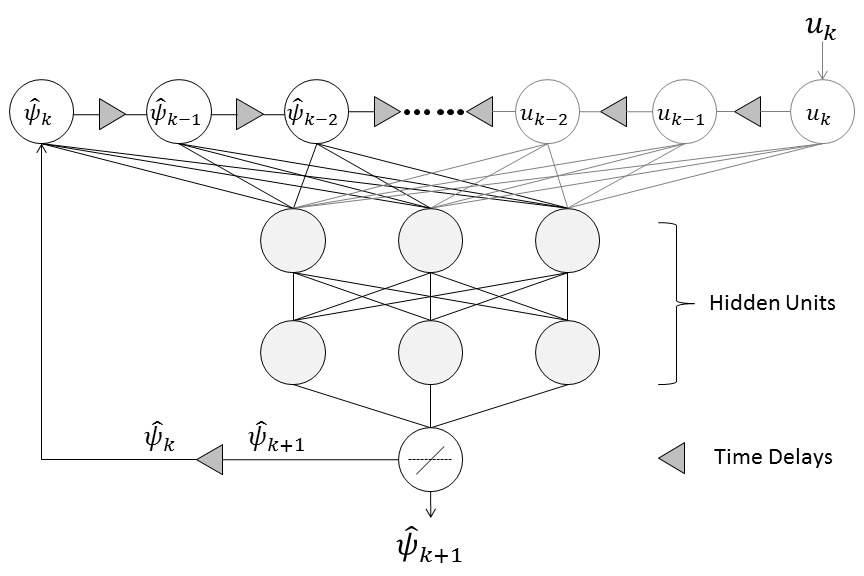
\includegraphics[width=1.0\textwidth]{narx_network_diagram.png}}
				\caption{Parallel NARX-network model with a linear output layer.}
				\label{fig::narx_net}
			\end{figure}
		%%%
		%%%

		\section{Potential-Fields Navigation}

		One method that has been selected for navigating the BlueFoot platform over flatland is a potential-fields control approach, described in \cite{Hogan1984} for the purpose of controlling robotic manipulators, and analyzed in-depth in \cite{Koren1991}. In particular \cite{Koren1991} presents shortcomings of this approach. Nonetheless, a potential fields navigation methods offers a relatively simple and intuitive approach to robot navigation and fits well into mobile robotic tasks which involve ``wandering'' type navigation over flat regions, in which the robot has yet to acquire any knowledge of surrounding obstacles. In this thesis, a potential fields navigation approach is used to navigate BlueFoot in unknown regions, and is coupled with camera-based feature tracking to guide the robot towards potential areas of interest within an unknown, immediate space.

		The potential fields approach is used in mobile robot navigation by moving the robot according to a guiding virtual force-vector, $F_{nav}$ \cite{Koren1991,ArambulaCosio2004}. This vector is comprised of a sum of virtual repulsive forces, $F^{-}$ (typically generated range-sensor data), and virtual attractive forces, $F^{+}$, which pull the robot towards known goals. Thus $F_{nav}$ formally defined as:
		%%%
		\begin{equation}
			F_{nav} = F^{+} + F^{-}
			\label{eq::sumofforces}
		\end{equation}

		The general form for the force components $F^{+}$ and $F^{-}$ (represented as $F_{c}$) is as follows:
		%%%
		\begin{eqnarray}
			d_{k} 	&=& p_{POI,k} - p_{robot} \nonumber\\
			F_{c}	&=& \alpha_{F}\sum_{k}\wrap{ f(\norm{d_{k}})\frac{d_{k}}{\norm{d_{k}}} }
			\label{eq::sumofforces}
		\end{eqnarray}	
		where $p_{poi}$ and $p_{robot}$ are position of each \Kth point-of-interest (POI) and the position of the robot platform; $f(*)$ is a potential function which returns a scalar ``energy" factor with respect to a scalar distance argument $(*)$; and $\alpha_{F}$ is a scaling parameter which is positive for when POIs represent goals and negative when POIs represent obstacles to avoid. The potential function and force-scaling factors are designable for particular applications. For BlueFoot's navigation scheme, attractive and repulsive forces are generated using a single, consolidated forcing function which is used to guide through an environment even when a goal is not specified before hand. 

		According to \cite{Koren1991} the main pitfall of a potential fields navigation approach is the hazard presented by local minima within the force global force-field. At a local minimum, the $F^{+}$ and $F^{-}$ are of nearly equal magnitude, causing the magnitude of the total guiding force vector $F_{c}$ to close to zero.  In practice, reaching a point at which robot will be completely stationary is an unlikely, as sensor readings used to observe environmental obstructions are corrupted by noise, which induce random perturbations under a potential-fields navigation regime. These perturbations could actually aid in relieving a situation in which a robot is stuck in a local minima. However, the gradient of the force-field around a minimum point could be very steep and cover a large area around the minima. These type of potential-sink regions cause the robot to exhibit limit-cycle behavior as it periodically overshoots and re-attracts to a nearby, singular force-minimum with a large relative pull. 

		This can be overcome, in part, by adding an artificial \emph{inertia} (essentially a tunable gain parameter) to robot navigation reference signals. Doing so may cause the robot platform to sufficiently overshoot a minimum point such that it leaves the local attraction field. A more sophisticated approach is mentioned in \cite{Krishnamurthy2007}, which involves a “stuck” detection algorithm. The idea behind such an algorithm involves a deduction about whether or not the robot is stuck within a local minima, based on samples of the robot’s motion state, and the execution of a small random-walk as a means of escape. Here, the local minima problem is addressed through the use of dynamic, auxiliary target points, as done in \cite{ArambulaCosio2004}. Here, however, a hybrid navigation scheme is used. Instead of incorporating goal points directly into the potential fields scheme, trackable features are handled using an entirely separate mode of navigation which is mixed with the base potential fields navigation scheme depending on a relative measure of ``closeness" to the object being tracked. The specifics of this will be describes in \ref{ch::navigation}. Hence, the potential-fields portion of this control scheme is used only for the purpose of avoiding potential obstructions, sensed via LIDAR range data. An image-feature tracking routine, based on visual-servoing, is used to guide the robot to features which fall within the robot’s camera gaze. This approach offers the ability to manually guide the robot during navigation, by either a human overseer, or a partner robot (which could wear trackable markers), as it performs an independent obstacle avoidance routine.The advantage of this approach lives in its simplicity, as it relies only on immediate environmental samples and, thus, has relatively minimal implementation demands.  As a mechanism for partially-guided wandering-type (random) navigation within an unknown region, this approach is certainly adequate as a will be shown via empirical results from both simulation and real-world trials.Surface Reconstruction for Rough Terrain NavigationThe previously introduced navigation scheme is utilizes for navigation of the BlueFoot platform over flatland and relies, largely, on 2D LIDAR scans.

		\section{3D Surface Reconstruction for Rough Terrain Planning}

		The previously introduced navigation scheme is utilizes for navigation of the BlueFoot platform over flatland and relies, largely, on 2D LIDAR scans. For navigation and planning over rough terrain, knowledge of 3D surfaces in the robot’s environment (with high feature detail) must be acquired. This thesis will provide the preliminaries for rough-terrain navigation and planning by way of several surface reconstruction methods from point-cloud data. First, a method for composing 3D point clouds from successive 2D LIDAR scans will be described. Then, algorithms for generating 3D height-maps and approximate surfaces from raw point-cloud data will be described. Finally, several component approaches for planning over the perceived terrain will be offered.


		\section{Overview of Thesis}

		This thesis will first detail the major hardware components; design considerations; and construction of the BlueFoot platform. Next, the software and processing architecture used to control the BlueFoot platform will be described. Thereafter, the kinematic and dynamical model of the BlueFoot system will be described, followed by control routines which are presently implemented to gait, stabilize, and navigate the BlueFoot platform. The final section of this thesis will contain concluding statement about the system design and control, including remarks about possible future directions of study related to the BlueFoot platform and legged robotics as a whole.
